\section{Locking on a narrow annulus}\label{sec:narrow}

Lemma~\ref{lem:fixed-locking} applies when one pair overlap exceeds a
fixed positive cutoff and the other two are close to zero. The path
argument also needs a different regime: the latter overlaps are near a
positive level $r$, while the first overlap exceeds $r$ by an amount
that may tend to zero. We obtain a uniform pressure loss for that regime.
Fix a minimizing measure $\mu$ and use its scalar data from
Section~\ref{static-sec:scalar}. Recall
$\Gamma(s)=\EE u(s,X_s)^2$, and write
$\chi_s=\chi(s,X_s)$. We work in the case where
$\Gamma(s)=s$ on a fixed interval; if the identity fails there, the pair
pressure gap supplies the forbidden interval used in
Section~\ref{sec:dynamics}.

Fix $t_0>0$ with $3t_0<q_*$, where $q_*$ is the constant in
Proposition~\ref{prop:coverage}. Recall $\rho=n^{-\kap}$ with
$\kap=1/10000$, and set
\begin{equation}\label{eq:narrow-scales}
 h=\rho^8,\qquad \varepsilon=\rho^{20}.
\end{equation}
Constants below may depend on $\beta,t_0$ and the fixed minimizing
measure. They do not depend on $n$ or on the overlap parameters.

The comparison will alter the fields by a contrast on the two sides
of a branching time, together with a short increment on the other
branch. When the surrounding interval has small Parisi mass, a tent
integration by parts shows that the contrast contributes little beyond
its Gaussian variance. The mixed term with the other branch then
provides the strict pressure loss.

\begin{lemma}[Narrow-annulus locking]\label{lem:narrow-locking}
Suppose that
\begin{equation}\label{eq:narrow-identity}
 \Gamma(s)=s\qquad\text{for }t_0/2<s<3t_0.
\end{equation}
For three independent Gibbs configurations $v,x,y$, conditionally on
the disorder, define
\[
 q=R(x,y),\qquad
 r=\frac{R(v,x)+R(v,y)}2,\qquad
 \delta=\frac{R(v,x)-R(v,y)}2.
\]
Then, for all sufficiently large $n$,
\begin{equation}\label{eq:narrow-locking-probability}
 \EE\pi^{\otimes3}\left\{
 \begin{array}{c}
 t_0/2<r<3t_0,\quad \mu([r-h,r+h])\le\rho^4,\\
 q\ge r+\rho,\quad \varepsilon\le|\delta|\le2\varepsilon
 \end{array}\right\}
 \le \exp(-n^{4/5}).
\end{equation}
\end{lemma}

\begin{proof}
Fix a feasible overlap matrix, in the coordinate order $v,x,y$,
\begin{equation}\label{eq:narrow-overlap-matrix}
 D=
 \begin{pmatrix}
 1&r+\delta&r-\delta\\
 r+\delta&1&q\\
 r-\delta&q&1
 \end{pmatrix},
\end{equation}
satisfying the event in~\eqref{eq:narrow-locking-probability}. We may
first impose the additional restriction
\begin{equation}\label{eq:narrow-pair-deviation}
 |q-\Gamma(q)|\le\rho^{13}.
\end{equation}
For an excluded pair overlap, \eqref{static-eq:pair-pressure} already gives a
pressure deficit of at least $\rho^{26}/2$. At the end of the proof
we will apply Lemma~\ref{lem:pressure-prob} to these deficits and sum
over the at most $n+1$ pair overlaps. The independent third draw does
not change their total probability.

For the minimizing scalar data, the source of the strict loss is already
visible. The identity
$\Gamma'(r)=1$ normalizes $\beta^2\EE\chi_r^2$ to one, whereas the
conditional susceptibility evolution decreases the mixed moment:
\[
 \beta^2\EE[\chi_q\chi_r]\le1-c(q-r).
\]
Step~8 will verify a uniform $c>0$. We construct a covariance
perturbation whose quadratic pressure change contains this deficit.
Its much larger Gaussian variance contribution will cancel against the
interpolation penalty.

The proof of the three-replica deficit has three stages. In
Steps~1--4 we construct an admissible perturbed hierarchy and reduce
the comparison to one quadratic moment. Steps~5--6 estimate that
moment using the tent on the first branch and a ramp on the second.
In Steps~7--9 we pass from finite hierarchies to the minimizing scalar
data, establish the negative quadratic coefficient, and sum the
resulting probability bounds.

\par\medskip\noindent\textbf{Step 1. Finite scalar data and the base hierarchy.}\enspace
For all large $n$, the overlap restrictions imply
\[
 0<r-h<r<r+h<q\le1.
\]
Take increasingly fine partitions of $[0,1]$ containing
$r-h,r,r+h,q$. On each half-open segment, approximate $\alpha$ by
its actual value at the left endpoint, and set its value at $1$ to
$1$. These approximations are nondecreasing step distribution
functions. They converge in $L^1$ and preserve the actual endpoint
values at the four indicated points. In particular, each satisfies
\begin{equation}\label{eq:narrow-step-oscillation}
 \alpha(r+h)-\alpha(r-h)\le\rho^4.
\end{equation}
During the finite calculations, we omit the approximation index:
$\alpha,\Phi,u,\chi,X,A$ mean the step data, and $\cP_\beta(\alpha)$ is
the scalar functional of the corresponding measure. These step
measures need not minimize the functional. We will use stationarity
only after passing to the minimizing limit.

We index only the integrated covariance increments: $Q_0=0$,
$Q_\ell-Q_{\ell-1}\succeq0$, with nondecreasing masses
$m_\ell\in[0,1]$ and field covariances
$\beta^2(Q_\ell-Q_{\ell-1})$. For this indexing write
\[
 Q_{\rm end}=Q_N,\qquad
 \int m\,\dd|Q|^2
 =\sum_{\ell=1}^N m_\ell
       (|Q_\ell|^2-|Q_{\ell-1}|^2).
\]
Prepending a zero-covariance quenched level gives precisely the
convention of Proposition~\ref{static-prop:matrix-bound}. We always use
zero terminal multiplier, so the terminal function is the sum of the
three scalar $\log(2\cosh)$ functions.

Build the base covariance path $Q$ in three stages:
\begin{enumerate}
 \item From scalar time $0$ to $r$, give all three fields the same
       increment of variance $\beta^2\,\dd s$, integrated at mass
       $\alpha(s)/3$.
 \item From $r$ to $q$, give $v$ its own scalar branch at mass
       $\alpha(s)$ and give $x,y$ a common scalar branch at mass
       $\alpha(s)/2$. The branches use independent Gaussian
       increments. Merge their finite schedules in nondecreasing
       mass order, preserving each branch's local order.
 \item From $q$ to $1$, give the three coordinates independent
       scalar increments simultaneously on each segment, all
       integrated at mass $\alpha(s)$.
\end{enumerate}
This is the base hierarchy of
Section~\ref{static-subsec:locking-base}, now with the specified finite
approximation. In the middle stage, scalar time is local to each branch:
we merge by mass, preserving each branch's order. The end masses of the
first stage are at most the starting middle masses, and the end middle
masses are at most the starting third-stage masses. Thus the complete
schedule is nondecreasing, and every increment is positive semidefinite.

Write $\Psi_0$ for its recursive value. The block-size cancellation
proved in Section~\ref{static-subsec:locking-base} gives
\begin{equation}\label{eq:narrow-base-value}
 \Psi_0-\frac{\beta^2}{4}\int m\,\dd|Q|^2
 =3\Phi(0,0)-\frac{3\beta^2}{2}\int_0^1s\alpha(s)\,\dd s
 =3\cP_\beta(\alpha).
\end{equation}
Its endpoint is $D$ with $\delta=0$. The same calculation identifies
the base tilted law: after the common path through $r$, the $x,y$
branch and the $v$ branch each have the scalar transition law. Denote
their scalar paths by $X^x$ and $X^v$; they coincide through $r$ and
then run to $q$ on their separate clocks. A frozen
branch's additive value cancels from every active normalized kernel,
so merging the schedules does not change their conditional independence.

To record the conditional independence that will be used below, let
$\mathcal X_0$ be the common prefix through $r$. If $K_{r,z}$ denotes
the scalar path law starting at $(r,z)$, then
\[
 \mathcal L(X^x_{[r,q]},X^v_{[r,q]}\mid\mathcal X_0)
 =K_{r,X_r}\otimes K_{r,X_r}.
\]
In particular, knowing the entire $x$ branch reveals no additional
future noise of the $v$ branch.

\par\medskip\noindent\textbf{Step 2. A perturbation preserving positive semidefiniteness.}\enspace
Set
\[
 \theta=\rho^2,\qquad a=1-\theta,
\]
and form the following linear combinations of field increments:
\begin{equation}\label{eq:narrow-Y}
 Y_0=\frac{(X^x_r-X^x_{r-h})-(X^x_{r+h}-X^x_r)}h,\qquad
 Y_1=\frac{X^v_{r+h}-X^v_r}h,\qquad
 Y=aY_0+\theta Y_1.
\end{equation}
Under the raw law these are Gaussian linear expressions. Under the
base tilted law the same expressions use the scalar paths just
identified. The contrast $Y_0$ includes the common increment before
the split and the $x$ increment after the split; $Y_1$ uses the
post-split increment on the $v$ branch. Figure~\ref{fig:narrow-increments}
shows these three increments and their covariance kernels.
\begin{figure}[t]
\centering
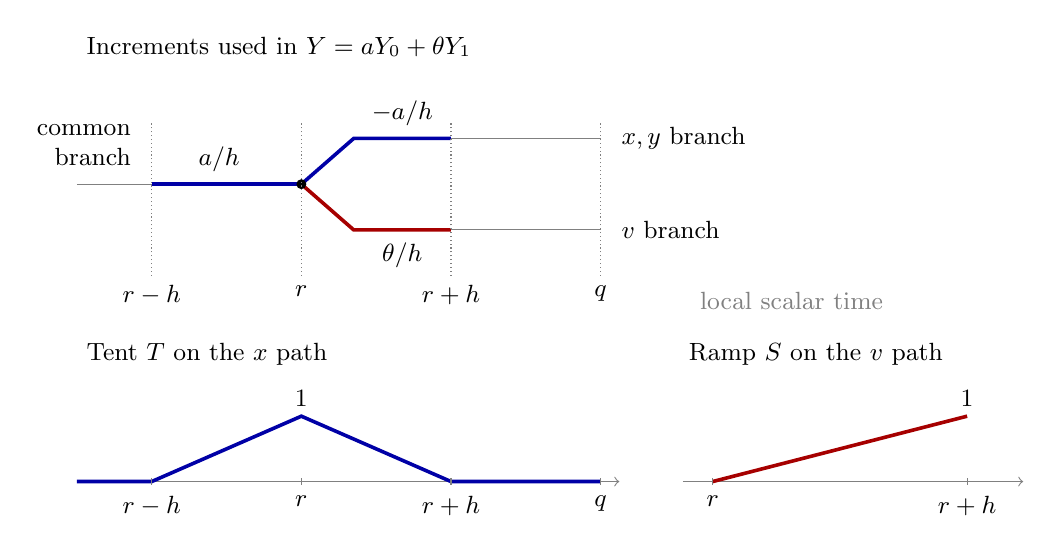
\begin{tikzpicture}[x=0.95cm,y=0.83cm,
  every node/.style={font=\small},
  active/.style={line width=1.3pt,blue!65!black},
  other/.style={line width=1.3pt,red!65!black}]
  \node[anchor=west] at (0,5.00) {Increments used in $Y=aY_0+\theta Y_1$};
  \draw[gray] (0,2.9)--(3,2.9);
  \draw[active] (1,2.9)--(3,2.9);
  \draw[active] (3,2.9)--(3.7,3.6)--(5,3.6);
  \draw[gray] (5,3.6)--(7,3.6);
  \draw[other] (3,2.9)--(3.7,2.2)--(5,2.2);
  \draw[gray] (5,2.2)--(7,2.2);
  \fill (3,2.9) circle[radius=1.8pt];
  \node[above] at (1.9,2.94) {$a/h$};
  \node[above] at (4.35,3.65) {$-a/h$};
  \node[below] at (4.35,2.15) {$\theta/h$};
  \node[anchor=west] at (7.15,3.6) {$x,y$ branch};
  \node[anchor=west] at (7.15,2.2) {$v$ branch};
  \node[anchor=east,align=right] at (0.85,3.50) {common\\branch};
  \foreach \x/\t in {1/{r-h},3/r,5/{r+h},7/q} {
    \draw[gray,densely dotted] (\x,1.5)--(\x,3.85);
    \node[below] at (\x,1.5) {$\t$};
  }
  \node[anchor=west,text=gray] at (8.2,1.12) {local scalar time};

  \node[anchor=west] at (0,0.30) {Tent $T$ on the $x$ path};
  \draw[->,gray] (0,-1.65)--(7.25,-1.65);
  \draw[active] (0,-1.65)--(1,-1.65)--(3,-0.65)
                       --(5,-1.65)--(7,-1.65);
  \node[above] at (3,-0.65) {$1$};
  \foreach \x/\t in {1/{r-h},3/r,5/{r+h},7/q} {
    \draw[gray] (\x,-1.60)--(\x,-1.70);
    \node[below] at (\x,-1.72) {$\t$};
  }

  \node[anchor=west] at (8.05,0.30) {Ramp $S$ on the $v$ path};
  \draw[->,gray] (8.1,-1.65)--(12.65,-1.65);
  \draw[other] (8.5,-1.65)--(11.9,-0.65);
  \node[above] at (11.9,-0.65) {$1$};
  \foreach \x/\t in {8.5/r,11.9/{r+h}} {
    \draw[gray] (\x,-1.60)--(\x,-1.70);
    \node[below] at (\x,-1.72) {$\t$};
  }
\end{tikzpicture}
\caption{The three increments in the perturbation. The upper labels are
coefficients of the raw field increments in $Y$; $a=1-\theta$.
Horizontal position records local scalar time, not the mass-sorted order
of the hierarchy. Below, the raw covariance of $Y_0$ with $X_s^x$,
divided by $\beta^2$, is the tent $T(s)$, which vanishes before the
endpoint $q$. Conditional on the common field $X_r$, the raw covariance
of $Y_1$ with $X_s^v$ on $[r,r+h]$, divided by $\beta^2$, is the ramp
$S(s)$. The tent isolates the small change in Parisi mass near $r$;
the other branch supplies the mixed susceptibility term. Lengths are
schematic.}
\label{fig:narrow-increments}
\end{figure}


At each level of the first two stages, add $\delta$ times that
level's contribution to $Y$ to the $x$ field, and subtract it from
the $y$ field. Leave $v$ unchanged. Each modified increment is a
deterministic linear image of its original Gaussian increment.
Consequently its covariance is positive semidefinite, and increments
at different levels remain independent. This gives an admissible
path $\widetilde Q$ with the original masses. At the end of the
second stage the added fields are $0,\delta Y,-\delta Y$.

For any prefix, write $K_c$ for the accumulated raw variance of
$Y$, divided by $\beta^2$, and write $g_v,g_x$ for its raw
covariances with the base $v,x$ fields in the same units. Its
covariance with the base $y$ field equals $g_x$. The coefficients
on the three active intervals are $a/h,-a/h,\theta/h$, so
\begin{equation}\label{eq:narrow-covariance-end}
 K=\frac{2a^2+\theta^2}{h},\qquad
 g_v^{\rm end}=a+\theta=1,\qquad g_x^{\rm end}=a-a=0.
\end{equation}
Let $e_v,e_x,e_y$ be the coordinate vectors and set
$L_2=(e_x-e_y)(e_x-e_y)^{\mathsf T}$. At every prefix,
\begin{equation}\label{eq:narrow-covariance-expansion}
 \widetilde Q=Q+\delta L_1+\delta^2K_cL_2,
 \qquad
 L_1=
 \begin{pmatrix}
 0&g_v&-g_v\\
 g_v&2g_x&0\\
 -g_v&0&-2g_x
 \end{pmatrix}.
\end{equation}
For the Frobenius product $U:V=\sum_{i,j}U_{ij}V_{ij}$, both $Q$
and $L_2$ are orthogonal to $L_1$. Also
$|L_1|^2=4g_v^2+8g_x^2$ and $|L_2|^2=4$. Expanding gives
\begin{equation}\label{eq:narrow-norm-expansion}
 |\widetilde Q|^2-|Q|^2
 =\delta^2\bigl(4g_v^2+8g_x^2+2K_c\,Q:L_2\bigr)
   +4\delta^4K_c^2.
\end{equation}
The endpoint is
\begin{equation}\label{eq:narrow-modified-end}
 \widetilde Q_{\rm end}=D+\delta^2K L_2.
\end{equation}
Its diagonal need not be one. We therefore use precisely the
arbitrary-endpoint comparison~\eqref{static-eq:matrix-bound}, proved
in Proposition~\ref{static-prop:matrix-bound}. It assigns the
endpoint discrepancy the cost
\begin{equation}\label{eq:narrow-mismatch}
 \frac{\beta^2}{4}|D-\widetilde Q_{\rm end}|^2
 =\beta^2\delta^4K^2.
\end{equation}

\par\medskip\noindent\textbf{Step 3. The penalty gain.}\enspace
We next compute the quadratic terms in the interpolation penalty.
The base $x,y$ fields coincide before the third stage, so $Q:L_2=0$
there. In the third stage, $Q:L_2=2(s-q)$ and $K_c=K$ is fixed.
The term $2K_c\,Q:L_2$ in~\eqref{eq:narrow-norm-expansion}
therefore contributes $\beta^2\delta^2K A(q)$ to the penalty.

For the other quadratic terms put
\[
 I=\int m\,\bigl(\dd(g_v^2)+2\dd(g_x^2)\bigr).
\]
The three active pieces have separate roles. Before the split, on
$[r-h,r]$, both covariances grow from $0$ to $a$ at mass
$\alpha(s)/3$; this contributes $\alpha(r)a^2+O(\rho^4)$.
On the active $v$ steps, $g_v$ grows from $a$ to $a+\theta$
and $g_x$ is fixed; this contributes
$\alpha(r)(2a\theta+\theta^2)+O(\rho^4)$.
On the active shared $x,y$ steps, $g_x$ decreases from $a$ to zero
and $g_v$ is fixed. The factor $2$ in $I$ cancels the factor
$1/2$ in their masses, giving $-\alpha(r)a^2+O(\rho^4)$.
The error in replacing each mass by $\alpha(r)$ is controlled by
\eqref{eq:narrow-step-oscillation} times the total variation of the
relevant covariance square. These total variations are uniformly
bounded, independently of the partition and its interleaving. Thus
\begin{equation}\label{eq:narrow-I}
 I=\alpha(r)(2a\theta+\theta^2)+O(\rho^4).
\end{equation}
Finally, $K_c$ is a nondecreasing cumulative variance and all masses
are nonnegative. The fourth-order contribution
$\int m\,\dd(K_c^2)$ is therefore nonnegative. Combining the terms
proves
\begin{equation}\label{eq:narrow-penalty}
 \frac{\beta^2}{4}\int m\,
       \dd\bigl(|\widetilde Q|^2-|Q|^2\bigr)
 \ge
 \beta^2\delta^2
 \bigl(KA(q)+\alpha(r)(2a\theta+\theta^2)-C\rho^4\bigr).
\end{equation}

\par\medskip\noindent\textbf{Step 4. The recursive-value cost.}\enspace
Let $\widetilde\Psi$ denote the modified one-site value. Integrating
the unchanged third stage backwards leaves the boundary difference
\begin{equation}\label{eq:narrow-U}
 U=\Phi(q,X_q^x+\delta Y)+\Phi(q,X_q^x-\delta Y)
                -2\Phi(q,X_q^x).
\end{equation}
Initially view this as a function of the full raw Gaussian prefix
through the second stage. Let $\EE_0$ denote expectation under its
base tilted law. We claim that
\begin{equation}\label{eq:narrow-recursive-comparison}
 \widetilde\Psi-\Psi_0\le\log\EE_0 e^U.
\end{equation}

Apply the normalized-kernel comparison
\eqref{static-eq:locking-recursive-sandwich} with boundary change $U$.
Here the state at each level is the entire raw Gaussian prefix: $Y$
uses several increments, so the current field alone need not determine
the modified future value. If $K_i$ is the normalized base kernel and
$\Delta_i$ is the change in recursive value, the ratio of the defining
integrals still gives
\[
 \Delta_i=\frac1{m_i}\log K_i e^{m_i\Delta_{i+1}}
 \quad(m_i>0),\qquad
 \Delta_i=K_i\Delta_{i+1}\quad(m_i=0).
\]
The kernel induction used for
\eqref{static-eq:locking-recursive-sandwich} therefore applies without
change and proves~\eqref{eq:narrow-recursive-comparison}. This argument
uses no inverse transformation of the fields, so singular covariance
increments cause no difficulty. Every kernel is from the base hierarchy,
whose tilted prefix law was identified in Step~1.

Write $\chi_q=\chi(q,X_q^x)$. By Lemma~\ref{static-lem:scalar-regularity},
\begin{equation}\label{eq:narrow-U-bounds}
 0\le U\le\delta^2Y^2,\qquad
 |U-\delta^2\chi_qY^2|\le C_\beta|\delta Y|^3.
\end{equation}
The diffusion representation under $\EE_0$ writes $Y=G+B_*$,
where $G$ is a centered Gaussian linear combination of Brownian
increments with variance $\beta^2K$, and $|B_*|\le C_\beta$.
Indeed, each drift in~\eqref{eq:narrow-Y} is bounded by
$\beta^2$, integrated for time $h$, and then divided by $h$.
No independence between $G$ and $B_*$ is required. Since
$\delta^2/h=O(\rho^{32})$, Gaussian exponential moments and
$|Y|\le|G|+C_\beta$ imply, for all large $n$,
\[
 \EE_0|Y|^3\le C_\beta h^{-3/2},\qquad
 \EE_0\!\left[Y^4e^{\delta^2Y^2}\right]\le C_\beta h^{-2}.
\]
Use $e^u\le1+u+\tfrac12u^2e^u$ for $u\ge0$, followed by
$\log(1+z)\le z$, and then~\eqref{eq:narrow-U-bounds}. We obtain
\begin{equation}\label{eq:narrow-exponential-error}
 \log\EE_0e^U
 \le \delta^2\EE_0[\chi_qY^2]
      +C_\beta\bigl(|\delta|^3h^{-3/2}+\delta^4h^{-2}\bigr).
\end{equation}

We have now reduced the comparison to estimating
$\EE_0[\chi_qY^2]$. Its Gaussian variance term will cancel the
$KA(q)$ part of the penalty up to the pair deviation. The strict
gain must come from the mixed moment of $Y_0$ and $Y_1$.

\par\medskip\noindent\textbf{Step 5. The tent on the first branch.}\enspace
We will establish the quadratic-moment bound
\begin{equation}\label{eq:narrow-quadratic}
 \EE_0[\chi_qY^2]
 \le\beta^2K\,\EE_0\chi_q
    +2a\theta\beta^4\alpha(r)\EE_0[\chi_q\chi_r]
    +C_\beta(\rho^4+\theta^2),
 \qquad \chi_r=\chi(r,X_r^x).
\end{equation}
Begin with the scalar $x$ path through $q$. Write its partition as
$0=s_0<\cdots<s_N=q$ and its scalar masses as
$m_j^{\rm sc}=\alpha(s_j)$. Its normalized tilted density $D_x$
relative to the raw Gaussian increments has logarithm
\begin{equation}\label{eq:narrow-density}
 \ell:=\log D_x
 =\sum_{j=0}^{N-1}m_j^{\rm sc}
    \bigl(\Phi(s_{j+1},X^x_{s_{j+1}})
                  -\Phi(s_j,X^x_{s_j})\bigr).
\end{equation}
The scalar masses appear here because the base-law factorization
in Step~1 has already canceled the divided matrix masses.

Let $T$ be the continuous piecewise linear tent supported on
$[r-h,r+h]$, zero at both endpoints and equal to one at $r$.
For functions of the raw cumulative coordinates, denote by
$\partial$ the derivative obtained by replacing $X^x_s$ with
$X^x_s+tT(s)$ and differentiating at $t=0$. Under the raw law,
\[
 {\rm Cov}_{\rm raw}(Y_0,X^x_s)=\beta^2T(s),\qquad
 {\rm Var}_{\rm raw}(Y_0)=\frac{2\beta^2}{h}.
\]
Finite-dimensional Gaussian integration by parts gives
\begin{equation}\label{eq:narrow-tent-ibp}
 \EE_{\rm raw}[Y_0f]=\beta^2\EE_{\rm raw}[\partial f],\qquad
 \EE_{\rm raw}[Y_0^2f]
 =\frac{2\beta^2}{h}\EE_{\rm raw}f
      +\beta^4\EE_{\rm raw}[\partial^2f].
\end{equation}
For a direct verification, multiply the Gaussian density by
$\exp\{tY_0-t^2(2\beta^2/h)/2\}$. This shifts every cumulative
coordinate by $t\beta^2T(s)$; one and two differentiations give
the two formulas. These derivatives act on raw coordinates, not
on the solution map of the tilted stochastic differential equation.

Telescope~\eqref{eq:narrow-density}. Since $T(0)=T(q)=0$,
only internal coefficients $m_{j-1}^{\rm sc}-m_j^{\rm sc}$ remain:
\[
 \partial\ell
 =\sum_{j=1}^{N-1}(m_{j-1}^{\rm sc}-m_j^{\rm sc})
          T(s_j)u(s_j,X^x_{s_j}),\qquad
 \partial^2\ell
 =\sum_{j=1}^{N-1}(m_{j-1}^{\rm sc}-m_j^{\rm sc})
          T(s_j)^2\chi(s_j,X^x_{s_j}).
\]
Only points strictly between $r-h$ and $r+h$ contribute. The sum
of the absolute coefficients at those points is at most
$\alpha(r+h)-\alpha(r-h)$. Thus
\begin{equation}\label{eq:narrow-density-derivatives}
 |\partial\ell|\le\rho^4,\qquad
 |\partial^2\ell|\le\rho^4.
\end{equation}
This estimate includes an atom at $r$. Atoms at $r-h$ or $r+h$
contribute zero because the tent vanishes there. No continuity of
$\alpha$ at these points is assumed.

The endpoint $q$ lies outside the tent, so $\partial\chi_q=0$.
Apply the second identity of~\eqref{eq:narrow-tent-ibp} to
$f=D_x\chi_q$:
\begin{align}
 \EE_0[\chi_qY_0^2]
 &=\frac{2\beta^2}{h}\EE_0\chi_q
   +\beta^4\EE_0\!\left[
         \chi_q\bigl((\partial\ell)^2+\partial^2\ell\bigr)\right]
 \notag\\
 &=\frac{2\beta^2}{h}\EE_0\chi_q+O_\beta(\rho^4).
 \label{eq:narrow-Y0-square}
\end{align}
At the tent's peak, put $u_r=u(r,X_r^x)$; then
$\partial u_r=\chi_r$. The first identity applied to
$f=D_x\chi_qu_r$ gives
\begin{align}
 \EE_0[\chi_qY_0u_r]
 &=\beta^2\EE_0[\chi_q\chi_r]
       +\beta^2\EE_0[\chi_qu_r\partial\ell]
 \notag\\
 &=\beta^2\EE_0[\chi_q\chi_r]+O_\beta(\rho^4).
 \label{eq:narrow-Y0-linear}
\end{align}
Both integrations by parts are legitimate for every fixed finite
partition. Scalar values grow at most linearly, their needed
derivatives are bounded, and the density grows at most
exponential-linearly in the finite Gaussian vector. Gaussian
integrability therefore justifies differentiation directly, or
after truncation and passage to the limit. The error estimates
above are uniform over the partitions.

\par\medskip\noindent\textbf{Step 6. The ramp on the other branch and the mixed moment.}\enspace
Condition now on the entire path $X^x$ through $q$. The product law
from Step~1 leaves the future $v$ branch as a scalar diffusion
starting at the fixed value $X_r$. On $[r,r+h]$, its conditional
tilted density has the form~\eqref{eq:narrow-density}, with starting
time $r$. Use the ramp $S(s)=(s-r)/h$ and denote the corresponding
raw-coordinate derivative by $\partial_v$. The raw covariance of
$Y_1$ with the cumulative coordinate at $s$ is $\beta^2S(s)$,
and its raw variance is $\beta^2/h$.

Let $\ell_v$ be this branch's conditional log density. Telescoping
its derivative produces the terminal term
$m_{\rm last}u(r+h,X^v_{r+h})$ and internal terms with total
absolute coefficient at most
$m_{\rm last}-m_{\rm first}\le1$. The initial value is fixed and
the ramp is zero there. Using $|u|\le1$ and $\chi\le1$ gives
\[
 |\partial_v\ell_v|\le2,\qquad
 |\partial_v^2\ell_v|\le2.
\]
The conditional second Gaussian integration-by-parts identity
therefore yields
\begin{equation}\label{eq:narrow-Y1-square}
 \EE_0[Y_1^2\mid X^x]
 =\frac{\beta^2}{h}
  +\beta^4\EE_0\!\left[
       (\partial_v\ell_v)^2+\partial_v^2\ell_v\mid X^x\right]
 =\frac{\beta^2}{h}+O_\beta(1).
\end{equation}
The error is uniform in the starting field $X_r$. Multiplying by
the $X^x$-measurable variable $\chi_q$ and averaging gives
\[
 \EE_0[\chi_qY_1^2]
 =\frac{\beta^2}{h}\EE_0\chi_q+O_\beta(1).
\]

For the mixed moment we need the conditional first moment of $Y_1$.
The Brownian increment has conditional mean zero. The arbitrary-start
martingale identity~\eqref{static-eq:scalar-martingale} gives
$\EE_0[u(z,X_z^v)\mid X^x]=u_r$, since the independent branch
starts at $X_r$. Hence its drift representation gives exactly
\begin{equation}\label{eq:narrow-Y1-mean}
 \EE_0[Y_1\mid X^x]
 =\frac{\beta^2}{h}\int_r^{r+h}
         \alpha(z)\EE_0[u(z,X^v_z)\mid X^x]\,\dd z
 =\beta^2\bar\alpha\,u_r,\qquad
 \bar\alpha=\frac1h\int_r^{r+h}\alpha(z)\,\dd z.
\end{equation}
Conditioning on the whole $x$ path introduces no additional
conditioning on the $v$ branch's future noise. Moreover,
\eqref{eq:narrow-step-oscillation} implies
$|\bar\alpha-\alpha(r)|\le\rho^4$. Since $Y_0,\chi_q,u_r$ are
$X^x$-measurable, combine~\eqref{eq:narrow-Y0-linear} with
\eqref{eq:narrow-Y1-mean} to obtain
\begin{equation}\label{eq:narrow-mixed}
 \EE_0[\chi_qY_0Y_1]
 =\beta^2\bar\alpha\,\EE_0[\chi_qY_0u_r]
 =\beta^4\alpha(r)\EE_0[\chi_q\chi_r]+O_\beta(\rho^4).
\end{equation}
Finally expand $Y^2=a^2Y_0^2+2a\theta Y_0Y_1+\theta^2Y_1^2$.
Equations~\eqref{eq:narrow-covariance-end},
\eqref{eq:narrow-Y0-square}, \eqref{eq:narrow-Y1-square}, and
\eqref{eq:narrow-mixed} prove~\eqref{eq:narrow-quadratic}.
The distinction between the two errors matters: the tent contributes
$O_\beta(\rho^4)$, while the ramp's $O_\beta(1)$ error is multiplied
by $\theta^2$.

\par\medskip\noindent\textbf{Step 7. Passing the pressure comparison to the minimizer.}\enspace
We can now apply~\eqref{static-eq:matrix-bound} to the modified finite
hierarchy. Combine the base value, mismatch, penalty, recursive
comparison, and moment estimates in
\eqref{eq:narrow-base-value}, \eqref{eq:narrow-mismatch},
\eqref{eq:narrow-penalty}, \eqref{eq:narrow-recursive-comparison},
\eqref{eq:narrow-exponential-error}, and
\eqref{eq:narrow-quadratic}. Since $K=O(h^{-1})$, the endpoint
cost is part of the $\delta^4h^{-2}$ error. Discard the additional
nonpositive term $-\beta^2\delta^2\alpha(r)\theta^2$ to get
\begin{align}
 F_{3,n}(D)\le 3\cP_\beta(\alpha)
 +\delta^2\bigl\{&
   \beta^2K(\EE_0\chi_q-A(q))
   +2a\theta\beta^2\alpha(r)
                    (\beta^2\EE_0[\chi_q\chi_r]-1)
   +C_\beta(\rho^4+\theta^2)\bigr\}
 \notag\\
 &\hspace{-1em}
   +C_\beta\bigl(|\delta|^3h^{-3/2}+\delta^4h^{-2}\bigr).
 \label{eq:narrow-step-pressure}
\end{align}
The constants do not depend on the partition.

Keep $n,r,q,\delta$ fixed and send the mesh size to zero.
Lemma~\ref{static-lem:scalar-regularity} gives uniform convergence
of the scalar derivatives and $L^1$ stability of the values. Couple
the diffusions with the same Brownian motion. Their drifts are
uniformly bounded and Lipschitz in space, so $L^1$ convergence of
$\alpha$ together with uniform convergence of $u$ gives path
convergence by Gronwall's inequality. The bounded expectations in
\eqref{eq:narrow-step-pressure} consequently converge. So do $A(q)$
and the scalar functional, the latter to $P_\beta$. By construction,
every approximation uses the actual value $\alpha(r)$.

This limit is taken at fixed $h$, so it requires no approximation
rate uniform as $h\downarrow0$. Returning to the minimizing data,
and writing $\EE$ for its scalar-process expectation, we have
\begin{align}
 F_{3,n}(D)\le 3P_\beta
 +\delta^2\bigl\{&
   \beta^2K(\EE\chi_q-A(q))
   +2a\theta\beta^2\alpha(r)
                    (\beta^2\EE[\chi_q\chi_r]-1)
   +C_\beta(\rho^4+\theta^2)\bigr\}
 \notag\\
 &\hspace{-1em}
   +C_\beta\bigl(|\delta|^3h^{-3/2}+\delta^4h^{-2}\bigr).
 \label{eq:narrow-pressure}
\end{align}
In the product $\chi_q\chi_r$, both susceptibilities belong to the
same scalar path. It remains to show that their evolution makes
the quadratic coefficient negative by more than all displayed
errors.

\par\medskip\noindent\textbf{Step 8. The strict quadratic margin and the scale choices.}\enspace
The assumed identity~\eqref{eq:narrow-identity} and the scalar
evolution imply
\[
 \beta^2\EE\chi_r^2=\Gamma'(r)=1.
\]
Multiply the conditional susceptibility identity
\eqref{eq:scalar-evolution} by $\chi_r$ and average. It gives
\begin{equation}\label{eq:narrow-susceptibility-loss}
 \beta^2\EE[\chi_q\chi_r]
 =1-\beta^4\int_r^q\alpha(z)\EE[\chi_z^2\chi_r]\,\dd z
 \le1-c(q-r)\le1-c\rho
\end{equation}
with a uniform $c>0$ over the allowed $r,q$. To justify uniformity,
including $q=1$, use the drift bound to obtain
$\sup_{s\le1}|X_s|\le\beta\sup_{s\le1}|B_s|+\beta^2$.
Choose a fixed $M$ so that the event that the right side is at most
$M$ has positive probability $p_M$. Continuity and strict positivity
of $\chi$ imply
\[
 c_M:=\min_{0\le s\le1,\ |z|\le M}\chi(s,z)>0.
\]
Thus $\EE[\chi_z^2\chi_r]\ge p_Mc_M^3$ for all the times under
consideration. Also $\alpha(z)\ge\alpha(t_0/2)>0$ when $z\ge r$.
We may take $c=\beta^4\alpha(t_0/2)p_Mc_M^3$ in
\eqref{eq:narrow-susceptibility-loss}. This argument uses positivity
on a compact set, not a lower bound for $\chi$ on the whole real
line.

The all-time stationarity identity~\eqref{eq:scalar-stationarity}
and the pair restriction~\eqref{eq:narrow-pair-deviation} give
\[
 \EE\chi_q-A(q)=\alpha(q)(q-\Gamma(q))\le\rho^{13}.
\]
Since $K=O(\rho^{-8})$, the first term in braces in
\eqref{eq:narrow-pressure} is at most $C_\beta\rho^5$.
For all large $n$, $a\ge1/2$; using
$\theta=\rho^2$, $\alpha(r)\ge\alpha(t_0/2)>0$, and
\eqref{eq:narrow-susceptibility-loss}, the second term is at most
$-c_1\rho^3$. The remaining brace term is $O_\beta(\rho^4)$.
The last two errors, after division by $\delta^2$, satisfy
\[
 C_\beta|\delta|h^{-3/2}\le C_\beta\rho^8,
 \qquad
 C_\beta\delta^2h^{-2}\le C_\beta\rho^{24}.
\]
Every positive error is therefore smaller than the negative
$\rho^3$ contribution for all large $n$. Uniformly over the
feasible matrices in question, this proves
\begin{equation}\label{eq:narrow-pressure-gap}
 F_{3,n}(D)\le3P_\beta-c_2\delta^2\rho^3
             \le3P_\beta-c_2\rho^{43}.
\end{equation}

\par\medskip\noindent\textbf{Step 9. From pressure deficits to the claimed probability.}\enspace
The choice $\kap=1/10000$ satisfies $43\kap<1/24$, so the deficit
in~\eqref{eq:narrow-pressure-gap} dominates the finite-size error
required by Lemma~\ref{lem:pressure-prob}. For each feasible triple
matrix that lemma gives two exponential bounds, with exponents at
least constant multiples of $n\rho^{43}$ and $n\rho^{86}$.
The latter equals $n^{1-86\kap}=n^{0.9914}$. Sum these bounds over
the at most $(n+1)^3$ triple overlap matrices.

For the pairs removed in~\eqref{eq:narrow-pair-deviation},
\eqref{static-eq:pair-pressure} and the same lemma give exponents at least
constant multiples of $n\rho^{26}$ and
$n\rho^{52}=n^{0.9948}$. There are at most $n+1$ pair overlaps
to sum over. The fixed constants and polynomial counts in both
sums are absorbed by $\exp(-n^{4/5})$ for all sufficiently large
$n$. This proves~\eqref{eq:narrow-locking-probability}.
\end{proof}
